\documentclass[a4paper]{article}

%%%%%%%% General %%%%%%%%%
\usepackage[utf8]{inputenc}
\usepackage{graphicx}
\usepackage{amsmath}
\usepackage{lscape}
\usepackage{makeidx}
\usepackage{subfiles}
\usepackage{lipsum}
\usepackage{multicol} % Permite escribir en dos columnas.
\usepackage[spanish]{babel}
\usepackage{csquotes}
\usepackage{siunitx} % Permite usar unidades del Sistema Internacional.
\usepackage[final]{pdfpages}


%%%%%%%% Referencias y links  %%%%%%%%
\usepackage{hyperref}
\hypersetup{
    colorlinks=true,
    linkcolor=blue,
    filecolor=magenta,      
    urlcolor=cyan
}

\usepackage{cleveref}

%%%%%%%% Dependencias para excel2latex %%%%%%%%%
\usepackage{booktabs} 
\usepackage{colortbl} 
\usepackage{multirow}
\usepackage{bigstrut}

%%%%%%%% Imagenes y bibliografía %%%%%%%%%
\usepackage{biblatex}
\addbibresource{bibliography/bib.bib}

%%%%%%%% Margenes APA %%%%%%%%%
\usepackage[lmargin=4cm, rmargin=2.5cm, tmargin=2.5cm, bmargin=2.5cm]{geometry}

%%%%%%%% Estilo de footers and headers %%%%%%%%%
\usepackage{fancyhdr} %Headers y footers
\pagestyle{fancy}
\fancyhf{}
\rhead{\textbf{Alumno: Franco Calvo}}
\lhead{\textbf{Vías de comunicación II}}
\rfoot{Página \thepage}

\begin{document}

\tableofcontents
\clearpage


\section{Dragalina}

\subsection{Generalidades}

\textbf{Definición:} es una máquina excavadora de grandes dimensiones que es 
ensamblada en el mismo lugar donde se va a usar. Sus usos generales son para 
minería y para el movimiento de grandes cantidades de material.

Estan formados por una grúa con una pluma de gran dimensión, dos tambres de cables,
los cuales son para elevar y arrastrar. Desde el cabla de elevación se sustenta
una cuchara que puede ser arrastrada por el cable de arrastre, como se ve en 
\Cref{fig:esquema_dragalina}

\href{https://www.youtube.com/watch?v=V4TK7boaxXM&t=8s}{Ejemplo de funcionamiento.}

\begin{figure}[ht]
  \centering
  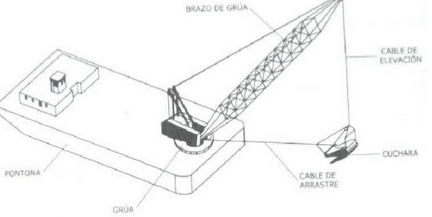
\includegraphics[width=0.8\textwidth]{../images/apuntes-presentacion-20210429/esquema_dragalina}
  \caption{Esquema de dragalina}
  \label{fig:esquema_dragalina}
\end{figure}

\subsection{Partes de la dragalina}

\subsubsection{Mecanismo de traslación}

El sistema de traslación puede variar, y define en gran medida el tamaño de la
dragalina.

\begin{description}
  \item[Sistema de oruga] son propulsadas por diésel, y consiste en un conjunto
    de eslabones que permiten el desplazamiento. Cuentan con varios ejes que 
    permiten el transporte como se ve en \Cref{oruga}, donde distinguimos lo 
    descrito a continuación. Un ejemplo de este sistema es 
    \href{https://www.youtube.com/watch?v=V4TK7boaxXM&t=8s}{este}.

    \begin{enumerate}
      \item Rueda de suspensión.
      \item Oruga.
      \item Rodillo de retorno.
      \item Rueda de trasmisión.
      \item Ruedas de rodadura.
      \item Rodillo tensión.
    \end{enumerate}

    \begin{figure}[ht]
      \centering
      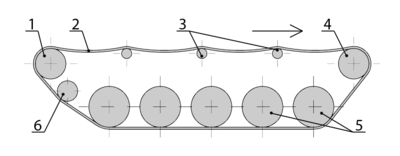
\includegraphics[width=0.5\textwidth]{../images/apuntes-presentacion-20210429/oruga}
      \caption{Esquema de oruga.}
      \label{fig:oruga}
    \end{figure}
  \item[Sistema de zapatas] este sistema es usado en sistemas de gran capacidad.
    Estas consisten en zapatas que mediante un sistema de engranajes puede hacer
    avanzar mediante acciones independientes de cada lado. 

    Su funcionamiento es el siguiente: primero se asientan las zapatas sobre el
    terreno, y luego se eleva el cuerpo de la máquina, y continua en un giro, haciendo
    un pequeño avance. Cuando se esta operando, las zapatas permanecen elevadas
    a alrededor de $\SI{0.5}{m}$ del suelo, como se ve en 
    éste \href{https://www.youtube.com/watch?v=-B_bRWVuITA}{video}.
    En \href{https://www.youtube.com/watch?v=iXDAXXRLupQ}{video} se puede ver el
    movimiento de la dragalina a partir del minuto 2:20.

\end{description}

\subsubsection{Bases de apoyo}

Pueden poseer una base de apoyo de forma circular y construcción cilíndrica recta
que transmite al terreno el peso de la máquina.

\subsubsection{Chasis giratorio}

Sobre ella se encuentra la plataforma de chasis giratorio sobre el que se encuentra
el resto de la máquina. En éste se encuentran los mecanismos de giro y los 
mecanismos de traslación.

\subsubsection{Bastidor en ángulo}

Es la estructura donde se encuentran fijados los cables de suspensión y la pluma.
Normalmente está constituida por dos pares devigas unidadas en el extremo, y donde
luego se encunetra fijado en la parte inferior por bulones.

\subsubsection{Mástil}

Es una estructura metálica de celosía desde donde se fijan los cables de la pluma.
Esto se une mediantembolunes al chasis.

\subsubsection{Pluma}

La pluma, que es lo que se encuentra suspendido por el mástil o el bastidor en
ángulo, se construye por vigas de celosía, y es la parte que define el alcance 
de la dragalina. 

\begin{figure}[ht]
  \centering
  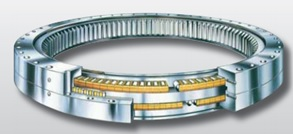
\includegraphics[width=0.45\textwidth]{../images/apuntes-presentacion-20210429/A3}
  \caption{Base de apoyo}
  \label{fig:A3}
\end{figure}


\subsection{Aplicaciones}

Las dragalinas tiene gran aplicación para la excavación y y transporte de suelos
a distancias de hasta $\SI{200}{m}$, dependiendo de la pluma de la máquina. 
Siempre excavan por debajo del nivel de apoyo, lo que permite eliminar el costo
de extracción de otros sistemas.Es muy aplicado para la construcción de canales
al excavar los taludes.

\subsection{Rendimiento}

Para excavaciones donde los suelos no son demasiado duros, su rendimiento es similar
a otros sistemas, pero a medida que aumenta la dureza su rendimiento baja ya que
no tiene demasiada penetración. La producción puede ser encontrada como:

\begin{align*}
  P_L = \frac{3600*C_b * F_w * E * FF * PT}{T_{CL}}
.\end{align*}

Donde $PL$ es la carga de producción,  $C_b$ la capacidad nominal de la cuchara,
 $F_w$ el factor de esponjamiento,  $E$ la eficacia operativa, $FF$ el factor
 de llenado, $PT$ el factor de posicionamineto y $T_{CL}$ el tiempo de ciclo por
 carga. 

\end{document}
